\section{Brugergrænseflade og design}
Af Kasper\\\\
Vores mål med programmet var at skabe en nemt og velfungerende måde at designe en carport på.
Det skulle føles intuitivt, og ikke skabe forvirring når man arbejder i programmet.
Programmet har været igennem flere forskellige stadier, før det nåede frem til vores endelige løsning.
\\
\subsection{Gennemgang af grænseflade}
\subsubsection{For brugere}
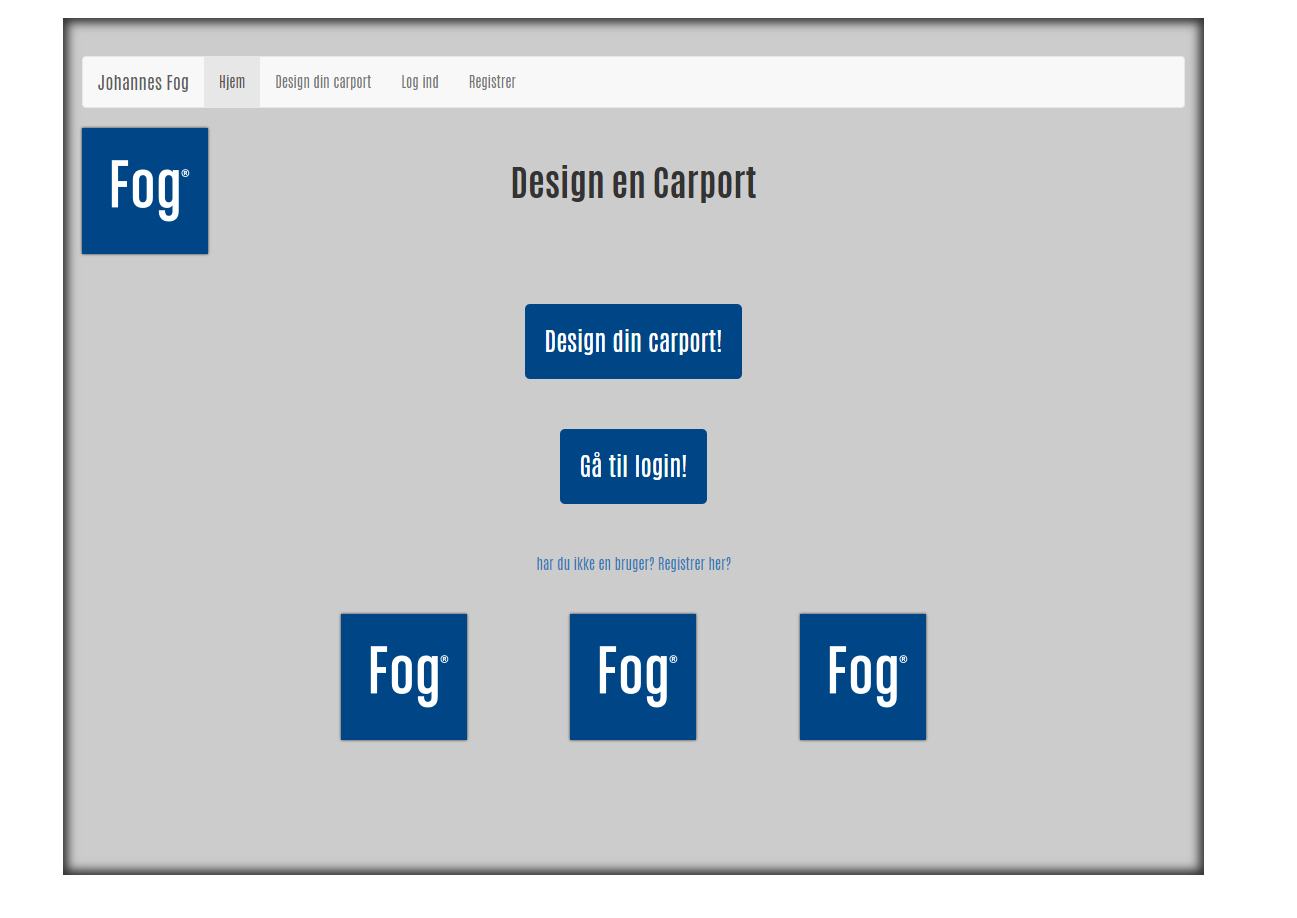
\includegraphics[width=\textwidth]{indexui}
Det første der skal tages stilling til for brugeren af siden er, om man vil logge in, registrere sig, eller bare prøve at designe sin carport.
Dette valg er bevidst stillet op for at tiltrække så mange potetientelle kunder som muligt.\\
Kunderne vil ikke som det første på siden oprette sig. Derfor får de muligheden for at arbejde med designværktøjet først, og gemme det senere.\\
Designmæssigt har vi ikke haft mulighed for at snakke med productowner Johannes Fog, og derfor har vi implementeret et design som er simpelt og nemt at finde rundt i.
Navigationsbaren i toppen kan bruges til at lede brugeren hen på den side de leder efter og har Johannes Fogs logo sat på.\\
\\\\
BILLEDE AF 3d
\\\\
Ved tryk på "design din carport"\ knappen ledes brugeren til vores 3D design program. Her kan brugeren køre sliders frem og tilbage, og vurdere hvordan deres carport skal se ud, og hvilke specifikke mål den skal have. Dette har den fordel at kunderne får en grafisk præsentation af hvordan deres carport kommer til at se ud, istedet for bare et billede af en tilfældig anden carport som firmaet engang. Når kunden føler at deres carport er som den skal være klikker de på "gem"\ knappen, og bliver herefter ledt videre til plantegningen af deres carport.
\\\\
BILLEDE AF 2D Her
\\\\
Her får kunden en 2D-plantegning af den carport de netop har designet i 3D-programmet. Tegningen har ikke alle mål sat på - dette er gemt til kunder der vælger at købe den carport de har designet. Samtidig med at tegningen er blevet genereret er carporten blevet gemt til brugeren, hvis man er logget ind. Hvis ikke, vil den bagefter bede dig om at logge in eller oprette dig.
\\\\
Billede af brugerpanel herefter
\\\\
Til slut kommer brugeren til brugerpanelet. Her kan de se den carport de har gemt, og kan trykke bestil, hvorefter ordren bliver sendt til databasen, til videre behandling af Fogs medarbejdere.
\subsubsection{for Fogs medarbejdere}
Fogs medarbejdere kan benytte dette samme system til behandling af ordrene. Hvis en medarbejder logger ind vil de blive taget til administratorpanelet. Her kan medarbejderne se status på de forskellige ordrer - om de er helt nye, under behandling af en kollega eller færdigbehandlet og klar til levering.
\\
Billede af Adminpanel her
\\

\subsection{Tekniske detajler}
Websiderne i projektet er skrevet i JSP, CSS og JavaScript, og benytter sig af JSTL og eksterne libraries så som THREE.js, jQuery og Bootstrap til at forbedre udseendet af projektet og gøre projeket kompatibelt med flere forskellige browsere og styresystemer. Så vidt muligt bliver disse libraries hentet eksternt, via et Content-Delivery Network (CDN). Dette skaber den fordel at brugerne kan have disse pakker cached fra tidligere brug på andre websider i forvejen, og derfor ikke behøver at hente dem igen. Det betyder også at pakkerne ikke kommer til at ligge på firmaets server, og derfor kan lette datatrafikken på serveren, og derved køre mere stabilt.\\
Workflowet er udarbejdet efter at kunne indsættes i et hvert webside-design, og til at kunne omskrives til andre programmeringssprog.\\
Dette giver os som gruppe muligheden for at udvikle i det sprog vi kender til (Java), samtidig med at det kan omskrives til, for eksempel, en C\# og ASP.Net baseret kodebase, hvilket er meget udbredt i Danmark.